\section{Geometric interpretation of eigenvectors}

Consider the matrix
\begin{equation*}
  A = \begin{mymatrix}{rr}
    2 & 1 \\
    1 & 2 \\
  \end{mymatrix}.
\end{equation*}
In Chapter~\ref{cha:linear-transformation}, we saw that this matrix
corresponds to a linear transformation $T : \R^2\to\R^2$ defined by
$T(\vect{x}) = A\vect{x}$. We also saw how to visualize this linear
transformation as a before-and-after picture. For this, we
considered the images of the first and second standard basis vectors,
which are the first and second column of $A$:
\begin{align*}
  T(\vect{e}_1) &= A\vect{e}_1 = \begin{mymatrix}{r} 2 \\ 1 \end{mymatrix},\\
  T(\vect{e}_2) &= A\vect{e}_2 = \begin{mymatrix}{r} 1 \\ 2 \end{mymatrix}.
\end{align*}
Here is the before-and-after picture for this transformation:
\vspace{-2cm}
\begin{center}
  \begin{tikzpicture}
    \begin{scope}[scale=0.4]
      \draw[red,thick,fill=red!10]
      (0,0) -- (0,5) -- (3,5) -- (3,4) -- (1,4) --
      (1,3) -- (2,3) -- (2,2) -- (1,2) -- (1,0) -- cycle;
      \draw[step=1cm, gray!50, very thin] (-5.8,-5.8) grid (5.8,5.8);
      \draw[red,thick]
      (0,0) -- (0,5) -- (3,5) -- (3,4) -- (1,4) --
      (1,3) -- (2,3) -- (2,2) -- (1,2) -- (1,0) -- cycle;
      \draw[semithick,->] (-6.5,0) -- (6.5,0);
      \draw[semithick,->] (0,-6.5) -- (0,6.5);
      \draw[blue,thick,->] (0,0) -- node[below] {$\vect{e}_1$} (5,0);
      \draw[blue,thick,->] (0,0) -- node[left] {$\vect{e}_2$} (0,5);
    \end{scope}
    \begin{scope}[xshift=3.6cm]
      \path (0,0) node {$\stackrel{T}{\longmapsto}$};
    \end{scope}
    \begin{scope}[xshift=7.2cm,scale=0.4]
      \draw[red,thick,fill=red!15,cm={2,1,1,2,(0,0)}]
      (0,0) -- (0,5) -- (3,5) -- (3,4) -- (1,4) --
      (1,3) -- (2,3) -- (2,2) -- (1,2) -- (1,0) -- cycle;
      \draw[step=1cm, gray!50, very thin] (-5.8,-5.8) grid (5.8,5.8);
      \draw[red,thick,cm={2,1,1,2,(0,0)}]
      (0,0) -- (0,5) -- (3,5) -- (3,4) -- (1,4) --
      (1,3) -- (2,3) -- (2,2) -- (1,2) -- (1,0) -- cycle;
      \draw[semithick,->] (-6.5,0) -- (6.5,0);
      \draw[semithick,->] (0,-6.5) -- (0,6.5);
      \draw[blue,thick,->,cm={2,1,1,2,(0,0)}] (0,0) --
      node[below right]
      {$T(\vect{e}_1) = \begin{mysmallmatrix}{r}2\\1\end{mysmallmatrix}$}
      (5,0);
      \draw[blue,thick,->,cm={2,1,1,2,(0,0)}] (0,0) --
      node[left,xshift=-0.1cm,pos=0.8]
      {$T(\vect{e}_2) = \begin{mysmallmatrix}{c}1\\2\end{mysmallmatrix}$}
      (0,5);
    \end{scope}
  \end{tikzpicture}
\end{center}
Although we can see from this picture that the letter ``F'' is being
distorted somehow, it is not so very obvious what exactly this linear
transformation is doing.

Now let us compute the eigenvectors and eigenvalues of $A$. A short
calculation shows that the eigenvectors are
\begin{equation*}
  \vect{v}_1 = \begin{mymatrix}{r} 1 \\ 1 \end{mymatrix}
  \quad\mbox{and}\quad
  \vect{v}_2 = \begin{mymatrix}{r} -1 \\ 1 \end{mymatrix},
\end{equation*}
with corresponding eigenvalues $\lambda_1=3$ and $\lambda_2=1$,
respectively. Consider the effect of the linear transformation $T$ on
the eigenvectors:
\begin{align*}
  T(\vect{v}_1) &= \begin{mymatrix}{rr}
    2 & 1 \\
    1 & 2 \\
  \end{mymatrix} \begin{mymatrix}{r} 1 \\ 1 \end{mymatrix}
  = \begin{mymatrix}{r} 3 \\ 3 \end{mymatrix}
  = 3\vect{v}_1, \\
  T(\vect{v}_2) &= \begin{mymatrix}{rr}
    2 & 1 \\
    1 & 2 \\
  \end{mymatrix} \begin{mymatrix}{r} -1 \\ 1 \end{mymatrix}
  = \begin{mymatrix}{r} -1 \\ 1 \end{mymatrix}
  = \vect{v}_2.
\end{align*}
So each eigenvector is mapped to a scalar multiple of itself. This
gives us a hint for how to draw a more useful before-and-after
picture. Rather than tracking the movement of the standard basis
vectors $\vect{e}_1$ and $\vec{e}_2$, let us track the movement of the
eigenvectors $\vect{v}_1$ and $\vect{v}_2$ instead:
\begin{center}
  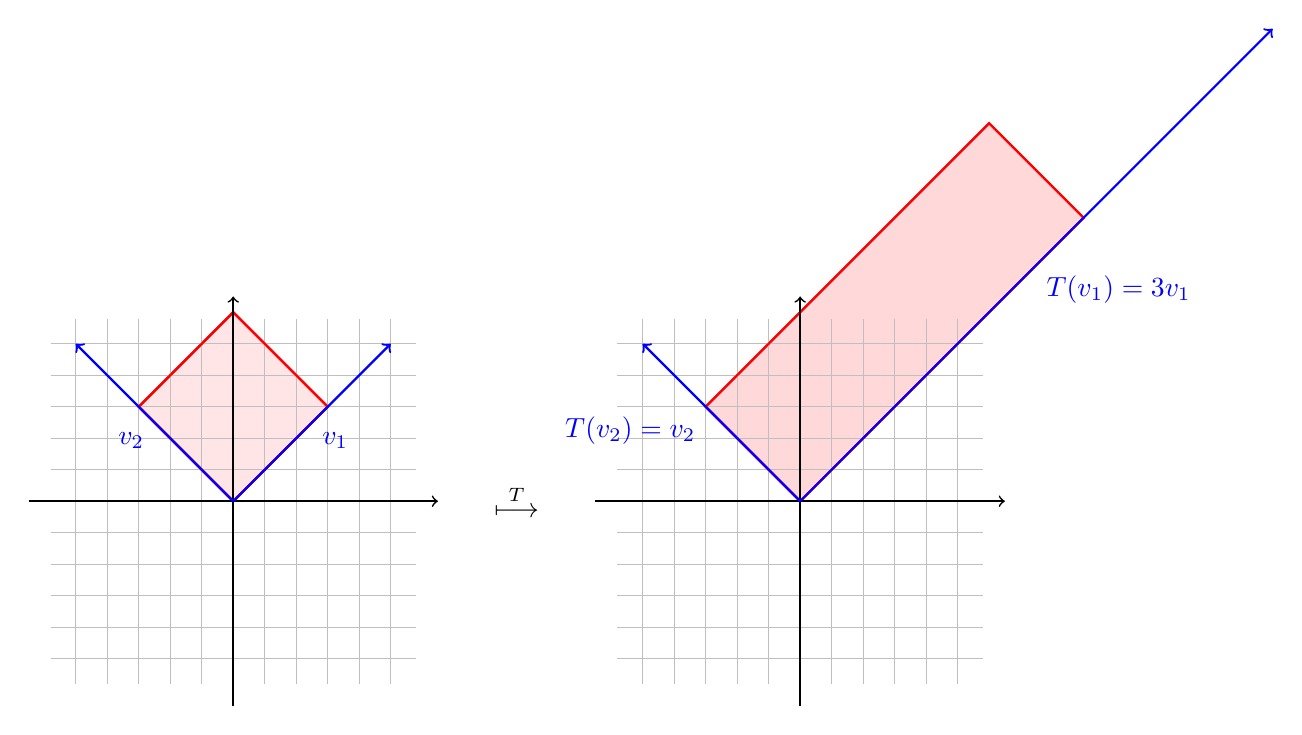
\begin{tikzpicture}
    \begin{scope}[scale=0.4]
      \draw[red,thick,fill=red!10]
      (0,0) -- (-3,3) -- (0,6) -- (3,3) -- cycle;
      \draw[step=1cm, gray!50, very thin] (-5.8,-5.8) grid (5.8,5.8);
      \draw[red,thick]
      (0,0) -- (-3,3) -- (0,6) -- (3,3) -- cycle;
      \draw[semithick,->] (-6.5,0) -- (6.5,0);
      \draw[semithick,->] (0,-6.5) -- (0,6.5);
      \draw[blue,thick,->] (0,0) -- node[below right] {$\vect{v}_1$} (5,5);
      \draw[blue,thick,->] (0,0) -- node[below left] {$\vect{v}_2$} (-5,5);
    \end{scope}
    \begin{scope}[xshift=3.6cm]
      \path (0,0) node {$\stackrel{T}{\longmapsto}$};
    \end{scope}
    \begin{scope}[xshift=7.2cm,scale=0.4]
      \draw[red,thick,fill=red!15,cm={2,1,1,2,(0,0)}]
      (0,0) -- (-3,3) -- (0,6) -- (3,3) -- cycle;
      \draw[step=1cm, gray!50, very thin] (-5.8,-5.8) grid (5.8,5.8);
      \draw[red,thick,cm={2,1,1,2,(0,0)}]
      (0,0) -- (-3,3) -- (0,6) -- (3,3) -- cycle;
      \draw[semithick,->] (-6.5,0) -- (6.5,0);
      \draw[semithick,->] (0,-6.5) -- (0,6.5);
      \draw[blue,thick,->,cm={2,1,1,2,(0,0)}] (0,0) --
      node[below right]
      {$T(\vect{v}_1) = 3\vect{v}_1$}
      (5,5);
      \draw[blue,thick,->,cm={2,1,1,2,(0,0)}] (0,0) --
      node[below left,pos=0.6]
      {$T(\vect{v}_2) = \vect{v}_2$}
      (-5,5);
    \end{scope}
  \end{tikzpicture}
\end{center}
Thus, the linear transformation described by the matrix $A$ is
revealed to be just a scaling by a factor of $3$ along the direction of
\begin{equation*}
  \vect{v}_1 = \begin{mymatrix}{r} 1 \\ 1 \end{mymatrix}.
\end{equation*}
